\documentclass[a4paper,preprint]{revtex4-2}
%\documentclass[aps,prl,preprint,superscriptaddress]{revtex4-2}
%\documentclass[aps,prl,reprint,groupedaddress]{revtex4-2}
% a4paper, amsfonts, amssymb, amsmath, preprint, superscriptaddress
\usepackage{amsfonts,amssymb,amsmath}
\usepackage{color}
\usepackage{csvsimple}
\usepackage{enumitem}
\usepackage{graphicx}
\usepackage[utf8]{inputenc} % allow utf-8 input
\usepackage{lineno}
\usepackage{microtype}      % microtypography
\usepackage{nicefrac}   

\newcommand{\pierre}[1]{{\color{red}Pierre: #1}}
\newcommand{\sref}[1]{S\ref{#1}}
\renewcommand{\eqref}[1]{Eq.~\ref{#1}}
\newcommand{\figref}[1]{Figure~\ref{#1}}
\newcommand{\SI}{Supplementary Material }

\newcommand{\Qmat}{\mathbf{Q}}
\newcommand{\papertitle}{Reconstruction of ancestral protein sequences using autoregressive generative models}

\begin{document}

\title{\papertitle}

\author{Pierre Barrat-Charlaix}
\email[Correspondance to: PBC, DISAT ]{pierre.barratcharlaix@polito.it}
\affiliation{DISAT, Politecnico di Torino, Italy}

\author{Matteo De Leonardis}
\affiliation{DISAT, Politecnico di Torino, Italy}

\author{Andrea Pagnani}
\affiliation{DISAT, Politecnico di Torino, Italy}

\date{}

\begin{abstract}
abstract
\end{abstract}

\maketitle


% !TEX root = main.tex

\section{Introduction}

\section{Results} % (fold)
\label{sub:results}

\subsection{Autoregressive model of sequence evolution} 
\label{sub:autoregressive_sequence_evolution_model}

Models of evolution commonly used in phylogenetics rely on the assumptions that sequence positions evolve independently and that evolution at each position $i$ follows a continuous time Markov chain (CTMC) parametrized by a substitution rate matrix $\Qmat^i$. 
Matrix $\Qmat^i$ is of dimensions $q \times q$ where $q=4$ for DNA, $20$ for amino acids or $64$ for codon models.
The probability of observing a change from state $a$ to state $b$ during evolutionary time $t$ is then given by $P(b \vert a, t) = \left( e^{t\Qmat^i} \right)_{ab}$.

If the model is time-reversible, it is a general property of CTMCs that the substitution rate matrix can be written as 

\begin{equation}
	\label{eq:Q_decomposition}
	\Qmat = \mathbf{H}\cdot \mathbf{\Pi} = \mathbf{H} \cdot \begin{pmatrix}
		\pi_1 & 0 & 0\\ 
		0 & \ddots & 0 \\
		0 & 0 & \pi_q
	\end{pmatrix},
\end{equation}

where $\mathbf{H}$ is symmetric and $\mathbf{\Pi}$ is diagonal with entries that sum to 1 \cite{yang_computationalmolecularevolution_2006}. 
The two matrices have simple interpretations. 
On the first hand, $\mathbf{\Pi}$ fixes the long-term equilibrium frequencies, that is $P(b \vert a, t) \xrightarrow[t \rightarrow \infty]{} \pi_b$.
On the other, $\mathbf{H}$ influences the dynamics of the Markov chain but does not change the equilibrium distribution. 
Most commonly, $\mathbf{\Pi}$ is considered to be independent of the sequence position $i$, while $\mathbf{H}$ can be multiplied by position-dependent rates in order to model the different variability of different sites \cite{yang_maximumlikelihoodphylogenetic_1994,stamatakis_raxmlversiontool_2014,nguyen_iqtreefasteffective_2015}. \\


In order to incorporate constraints coming from a protein's structure and function into the evolutionary model, we develop a family-specific model of protein sequence evolution based on the the autoregressive generative model ArDCA \cite{trinquier_efficientgenerativemodeling_2021}. 
ArDCA models the diversity of sequences in a protein family using a set of learned conditional probabilities. 
In practice, the model assigns a probability to any sequence $\mathbf{a} = \{a_1, \ldots, a_L\}$ of $L$ amino acids: 

\begin{equation}
	\label{eq:autoregressive_def}
	P^{AR}(\mathbf{a}) = \prod_{i=1}^L p_i(a_i \vert a_{<i}),
\end{equation}

where the product runs over positions in the sequence and $a_{<i} = a_1, \ldots, a_{i-1}$ represents all amino acids before position $i$. 
Functions $p_i$ represent the probability according to the model to observe state $a_i$ in position $i$, given that the previous amino acids were $a_1, \ldots, a_{i-1}$. 
Their precise functional form is given in the methods section. 
They are learned using the aligned sequences of members of the family. 
In actual implementations, the order in which the product in \eqref{eq:autoregressive_def} is performed is not the natural $(1, \ldots, L)$ but rather an order where positions are sorted by increasing variability.
This does not significantly effect the model we present below, and we keep the notation of \eqref{eq:autoregressive_def} for simplicity. 

It has been shown in \cite{trinquier_efficientgenerativemodeling_2021} that the generative capacities of ArDCA are comparable to that of state of the art models such as bmDCA \cite{mcgee_generativecapacityprobabilistic_2021}. 
This means that a set of sequences sampled from the probability in \eqref{eq:autoregressive_def} is statistically hard to distinguish from the natural sequences used in training or, in other words, that the model can be used to sample new artificial homologs of a protein family. 
Generative capacities of a protein model come from its ability to represent epistasis, that is the relation between the effect of a mutation and sequence context in which it occurs. 
Here, epistasis is modeled through the conditional probabilities $p_i$: the distribution of amino acids at position $i$ depends on the states of the previous positions $1, \ldots i-1$. 


We take advantage of the autoregressive architecture to define the following evolution model. 
Given two amino acid sequences $\mathbf{a}$ and $\mathbf{b}$, we propose

\begin{equation}
	\label{eq:autoregressive_propagator_full}
	P(\mathbf{b} \vert \mathbf{a}, t) = \prod_{i=1}^L q_i(b_i \vert a_i, b_{<i}, t),
\end{equation}

where the conditional propagator $q_i$ is defined as 

\begin{equation}
	\label{eq:autoregressive_site_propagator}
	q_i(b_i \vert a_i, b_{<i}, t) = \left(e^{t \cdot Q^i(b_{<i})}\right)_{a_i, b_i}, 
	\quad Q^i(b_{<i}) = \mathbf{H} \cdot \begin{pmatrix}
		p_i(1 \vert b_{<i}) & 0 & 0\\ 
		0 & \ddots & 0 \\
		0 & 0 & p_i(q \vert b_{<i})
	\end{pmatrix}. 
\end{equation}

According to these equations, evolution for each position $i$ follows a standard CTMC. 
However, we use the decomposition of \eqref{eq:Q_decomposition} to set the equilibrium frequency at $i$ to $p_i(b \vert b_{<i})$. 
In other words, we consider that position $i$ evolves in the context of $b_1, \ldots, b_{i-1}$, and that its dynamics are constrained by its long term frequency given by the autoregressive model. 
An important consequence of this choice is that our evolution model will converge at long times to the generative distribution $P^{AR}$: 

\begin{equation}
	\label{eq:autoregressive_long_term}
	q_i(b_i \vert a_i, b_{<i}, t) \xrightarrow[t \rightarrow \infty]{} p_i(b_i \vert b_{<i}), 
	\;\; P(\mathbf{b} \vert \mathbf{a}, t) \xrightarrow[t \rightarrow \infty]{} P^{AR}(\mathbf{b}).
\end{equation}

We argue here that such a property is essential to build a realistic protein sequence evolution model, particularly when considering evolution over a relatively long time frame. 
Note that to converge to a generative distribution, accurate modeling of epistasis is required. 
Using site-specific frequencies would not be sufficient, as the effect of mutations in a protein sequence typically depends on the context \cite{socolich_evolutionaryinformationspecifying_2005}. 
The technique proposed here allows us to represent epistasis through the context dependent probabilities $p_i$, while still considering each sequence position one at a time. 

Interestingly, we note that the model in \eqref{eq:autoregressive_propagator_full} is not time reversible, although context dependent site propagators in \eqref{eq:autoregressive_site_propagator} are reversible. 
We show in the SM that this is mainly an artifact of the autoregressive nature of the model coupled with epistasis. 
Using non-time reversible evolutionary models is uncommon in the field, but this is mainly due to practical considerations and there are no fundamental reasons for evolution itself to be reversible \cite{felsensteinjoseph_inferringphylogenies_2003}. 
In practice, this means that algorithms using this model have to be adapted accordingly. \\


We underline that this approach has important differences with standard models of evolution used in phylogenenetics. 
In phylogenetic reconstruction, the tree and the sequence evolution model are usually inferred at the same time and from the same data. 
The number of parameters of the evolution model is then kept low to reduce the risk of overfitting, for instance by using site specific rates to account for variable and conserved sites. 
Methods that introduce more complex models such as site specific frequencies do so by jointly inferring the parameters and the tree, leading to relatively complex algorithms \cite{halpern_evolutionarydistancesproteincoding_1998a,puller_efficientinferencepotential_2020}.

Here instead, parameters of the generative model in \eqref{eq:autoregressive_def} are learned from a protein family, \emph{i.e.} a set of diverged homologous protein sequences. 
While it is true that these sequences share a common evolutionary history and cannot be considered as independent samples, common learning procedures only account for this in a very crude way \cite{cocco_inversestatisticalphysics_2018,trinquier_efficientgenerativemodeling_2021}.
Despite this, it appears that the generative properties of such models are not strongly affected by ignoring the phylogeny \cite{hockenberry_phylogeneticweightingdoes_2019,rodriguezhorta_effectphylogeneticcorrelations_2021}. 
This allows us to proceed in two steps: first construct the model from data while ignoring phylogeny, and then only use it for phylogenetic inference tasks.

An advantage of this approach is that once the model of \eqref{eq:autoregressive_def} is inferred, the propagator in \eqref{eq:autoregressive_propagator_full} comes ``for free'' as no additional parameters are required. 
Importantly, our model does not use site specific substitution rates. 
Indeed, it has been shown that these can be seen as emergent properties when using more complex evolution models such as the one presented here \cite{delapaz_epistaticcontributionspromote_2020}.
However, a disadvantage is that the technique is only applicable to a given protein family at a time, and requires the existence of an appropriate training set for the model. 


\subsection{Ancestral sequence reconstruction}

We apply our evolutionary model to the task of ancestral sequence reconstruction (ASR). 
The goal of ASR is the following: given a set of extant sequences with a shared evolutionary history and the corresponding phylogenetic tree, is it possible to reconstruct the sequences of extinct ancestors at the internal nodes of the tree? 
Along with the autoregressive evolutionary model described above, we thus need two inputs to perform ASR: a known phylogenetic tree, and the multiple sequence alignment of the leaf sequences. 
The length of the aligned sequences has to exactly correspond to that of the autoregressive model. 

To reconstruct ancestral sequences using the autoregressive model, we proceed as follows: 
\begin{enumerate}[label=\emph{\roman*}]	
	\item for sequence position $i=1$, use the evolution model defined by the equilibrium frequencies $p_1$ to reconstruct a state $a^n_1$ at each internal node $n$ of the tree;
	\item iterating through subsequent positions $i > 1$: reconstruct state $a^n_i$ at each internal node $n$ using the model defined in \eqref{eq:autoregressive_site_propagator}, with the context $a^n_{<i}$ having been already reconstructed in the previous iterations. 
\end{enumerate}
It is important to note that when any position $i>1$ is reconstructed, the context at different internal nodes of the tree may differ. 
For a branch joining two nodes $(n, m)$ of the tree, the evolution model will thus differ if we go down or up the branch: in one case the context at node $n$ must be used, in the other case the context at node $m$. 
This is a consequence of the time-irreversibility of the model. 
For this reason, we use a variant of Felsenstein's pruning algorithm that is adapted to irreversible models \cite{boussau_efficientlikelihoodcomputations_2006}. 
This comes at no computational cost. 

Note that this method is adapted to both maximum likelihood and Bayesian inference. 
In the ML case, each iteration reconstructs the most probable residue is at a position $i$ given the already reconstructed context. 
In the Bayesian case, residue $a^n_i$ is instead sampled from the posterior distribution. 

In any realistic application, the phylogenetic tree has to be reconstructed from the aligned sequences. 
In principle, a consistent approach would use the same evolutionary model for tree inference and ASR. 
However, our model does not allow us to reconstruct the tree.
Therefore, in any realistic application, the tree is reconstructed using an evolutionary model that typically will differ from ours. 

To reduce issues related to this evolutionary model discrepancy, we adopt the following strategy: our ASR method blindly trusts the topology of the input tree, but recomputes the branch length using the sequences. 
As explained in the Methods, there is no direct way to optimize branch length with the autoregressive model. 
For simplicity, we use profile model with position-specific amino acid frequencies for this task. 
This provides a relatively accurate estimate of the branch lengths, as shown in Figure~\sref{sfig:branch_length_reconstruction}.


\subsection{Results on simulated data}

\paragraph*{Setup.} There are two difficulties when evaluating the capacity of a model to perform ASR. 
The first is that in the case of biological data, the real phylogeny and ancestral sequences are usually not known. 
As a consequence, one must rely on simulated data to measure the quality of reconstruction. 
The second is that the reconstruction of an ancestral sequence is always uncertain, as evolutionary models are typically stochastic. 
The uncertainty becomes higher for nodes that are remote from the leaves.
This means that it is only possible to make a statistical assessment about the quality of a reconstruction. 

To test our approach, we adopt the following setup. 
We first generate phylogenetic trees by sampling from a coalescent process.
We decide to use Yule's coalescent instead of the more common Kingman.
The latter tends to produce a large majority of internal nodes in close vicinity to the leaves with the others separated by very long branches, resulting in a trivial reconstruction for most nodes and a very hard one for the deep nodes. 
Yule's coalescent generates a more even distribution of node depths, allowing us to better evaluate reconstruction quality, see \SI  and Figure~\sref{sfig:depth_distribution_coalescent}.
For each tree, we simulate the evolution of sequences using a model that we refer to as ``evolver'' to obtain two multiple sequence alignments, one for the leaves and one for the internal nodes of the tree.
We then reconstruct internal nodes using the desired approach by using the leaf alignment and the tree topology as input data. 

We will consider two kinds of evolver models: \emph{(i)} the same autoregressive model that we will then use for reconstruction, which is an ideal case and \emph{(ii)} an evolutionary model based on a Metropolis sampling of a Potts model. 
These two evolvers come from models trained on actual protein families: we use evolvers based on the PF00072 response regulator family for results of the main text, and show results for three other families (PF00014, PF00076 and PF00595) in the \SI.  
It is important to note that the approach that we propose only makes sense when considering the evolution of a precise protein family, on which the model in \eqref{eq:autoregressive_def} is trained. 
Hence, any evolver model used in our simulations should reproduce at long times the statistics of the considered protein family, \emph{i.e.} it should satisfy \eqref{eq:autoregressive_long_term}. 
For this reason, we only consider the two evolvers above and do not use more traditional evolutionary models such as an arbitrary GTR on amino-acids \cite{rambaut_seqgenapplicationmonte_1997}. 

For reconstruction, we compare our autoregressive approach to the commonly used IQ-TREE program  \cite{minh_iqtreenewmodels_2020}.
When supplied with a protein sequence alignment and a tree, IQ-TREE infers a joint substitution rate matrix for all sequence positions, with rates that can differ accross positions. 
Both methods run on a fixed tree topology, with branch lengths being re-inferred using maximum likelihood (see Methods). \\

\begin{figure}
	\centering
	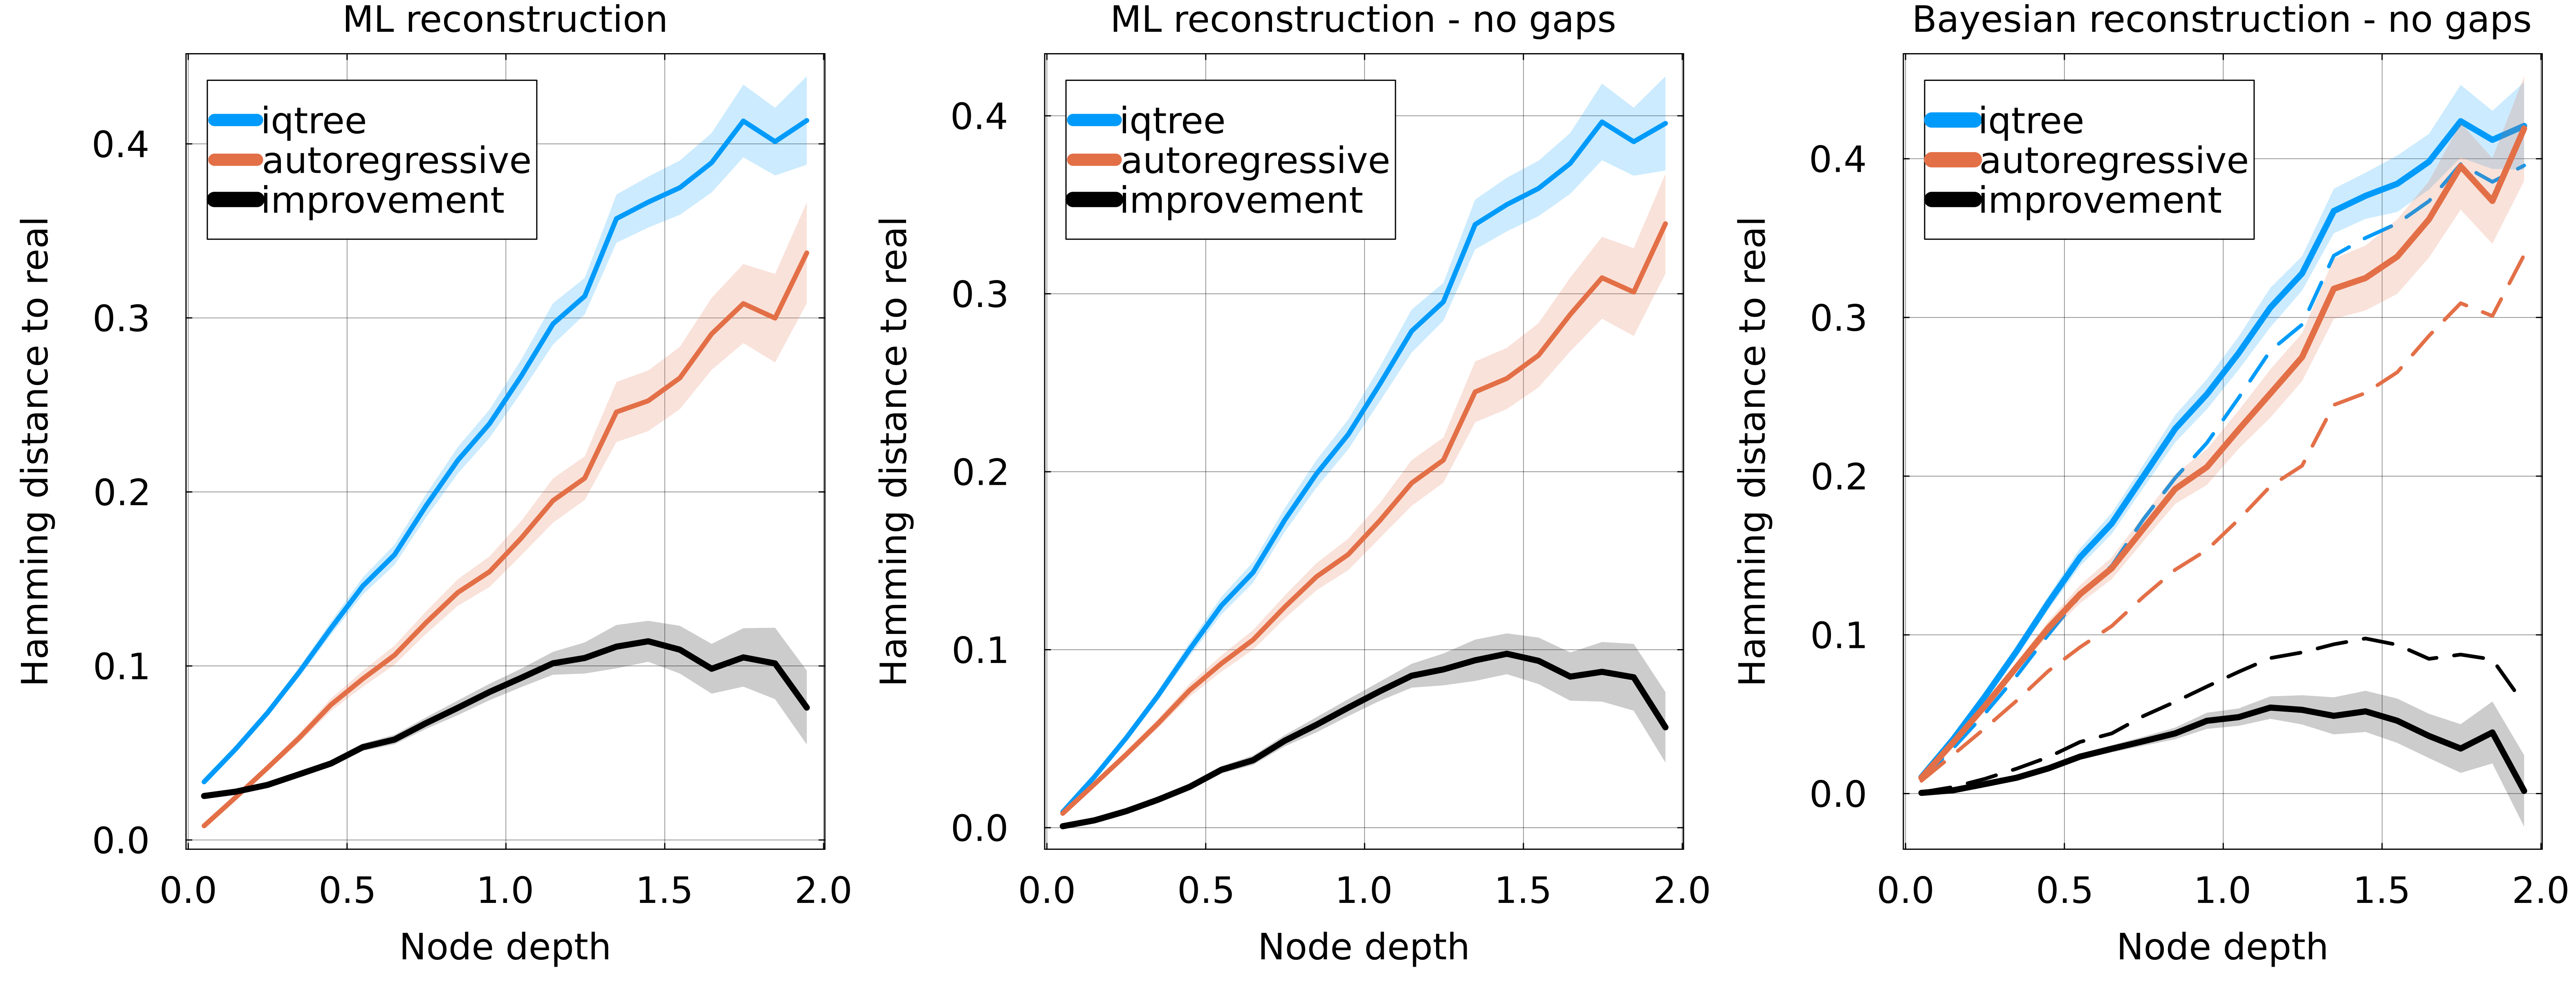
\includegraphics[width = \textwidth]{figures/hamming_to_real_arnet_PF00072.png}
	\caption{
		Hamming distance between reconstructed and real sequences as a function of node depth, using IQ-TREE and our autoregressive approach. 
		The difference between the two methods (``improvement'') is shown as a black curve. 
		Estimation of the incertitude is shown as a ribbon. 
		The evolver and reconstruction autoregressive models are learned on the PF00072 family. 
		\textbf{Left}: Hamming distance between the full aligned sequences, gaps included, using maximum likelihood reconstruction.  	
		\textbf{Center}: Hamming distance ignoring gapped positions, using maximum likelihood reconstruction. 
		\textbf{Right}: comparison of Bayesian (solid lines) and maximum likelihood (dashed lines) reconstructions, ignoring gaps. 
	}
	\label{fig:hamming_real_arnet}
\end{figure}

\paragraph*{Autoregressive evolver.} We first investigate the case of the autoregressive evolver. 
This setting is of course ideal for our method, as there is perfect coincidence between the model used to generate the data and to perform ASR. 
We first evaluate the quality of reconstruction by computing the Hamming distance of the real and inferred sequences for each internal node of the simulated phylogenies. 
The left and central panels of \figref{fig:hamming_real_arnet} show this Hamming distance as a function of the node depth, that is the distance separating the node from the leaves, and for a maximum likelihood reconstruction. 
Hamming distance is computed including gap characters in the aligned sequences on the right panel, while they are ignored on the central one. 
We see that the autoregressive reconstruction clearly outperforms the state of the art method: the improvement in Hamming distance increases with node depths, and the distance to the real ancestor drops from $\sim 0.4$ to $\sim 0.3$ when using the autoregressive approach. 

Interestingly, the performance of IQ-TREE degrades if Hamming distance is computed including gaps, as in the left panel. 
This is because like other popular methods, IQ-TREE treats gaps in input sequences as unknown amino acids, and reconstructs an ancestral amino acid for gapped positions \cite{yang_pamlphylogeneticanalysis_2007,minh_iqtreenewmodels_2020}. 
On the contrary, our autoregressive approach treats gaps as if they were an additional amino acid and will reconstruct ancestral sequences that can contain gaps. 
This benefits the autoregressive approach as aligned ancetral sequences can in fact contain gaps.
This effect is particularly visible at low node depths. 
However, ignoring the effects of gaps in the Hamming distance also leads to a clear improvement when using the autoregressive approach as shown in the central panel. 

The right panel of \figref{fig:hamming_real_arnet} shows the quality of the reconstruction for Bayesian reconstruction. 
In this case, a ensemble of sequences is reconstructed for each internal node, and the metric is the average Hamming distance between this ensemble and the real ancestor. 
Gaps are again ignored when computing the Hamming distance. 
We again observe an improvement when using the autoregressive method, of slightly lesser magnitude than in the maximum likelihood case. \\


\begin{figure}
	\centering
	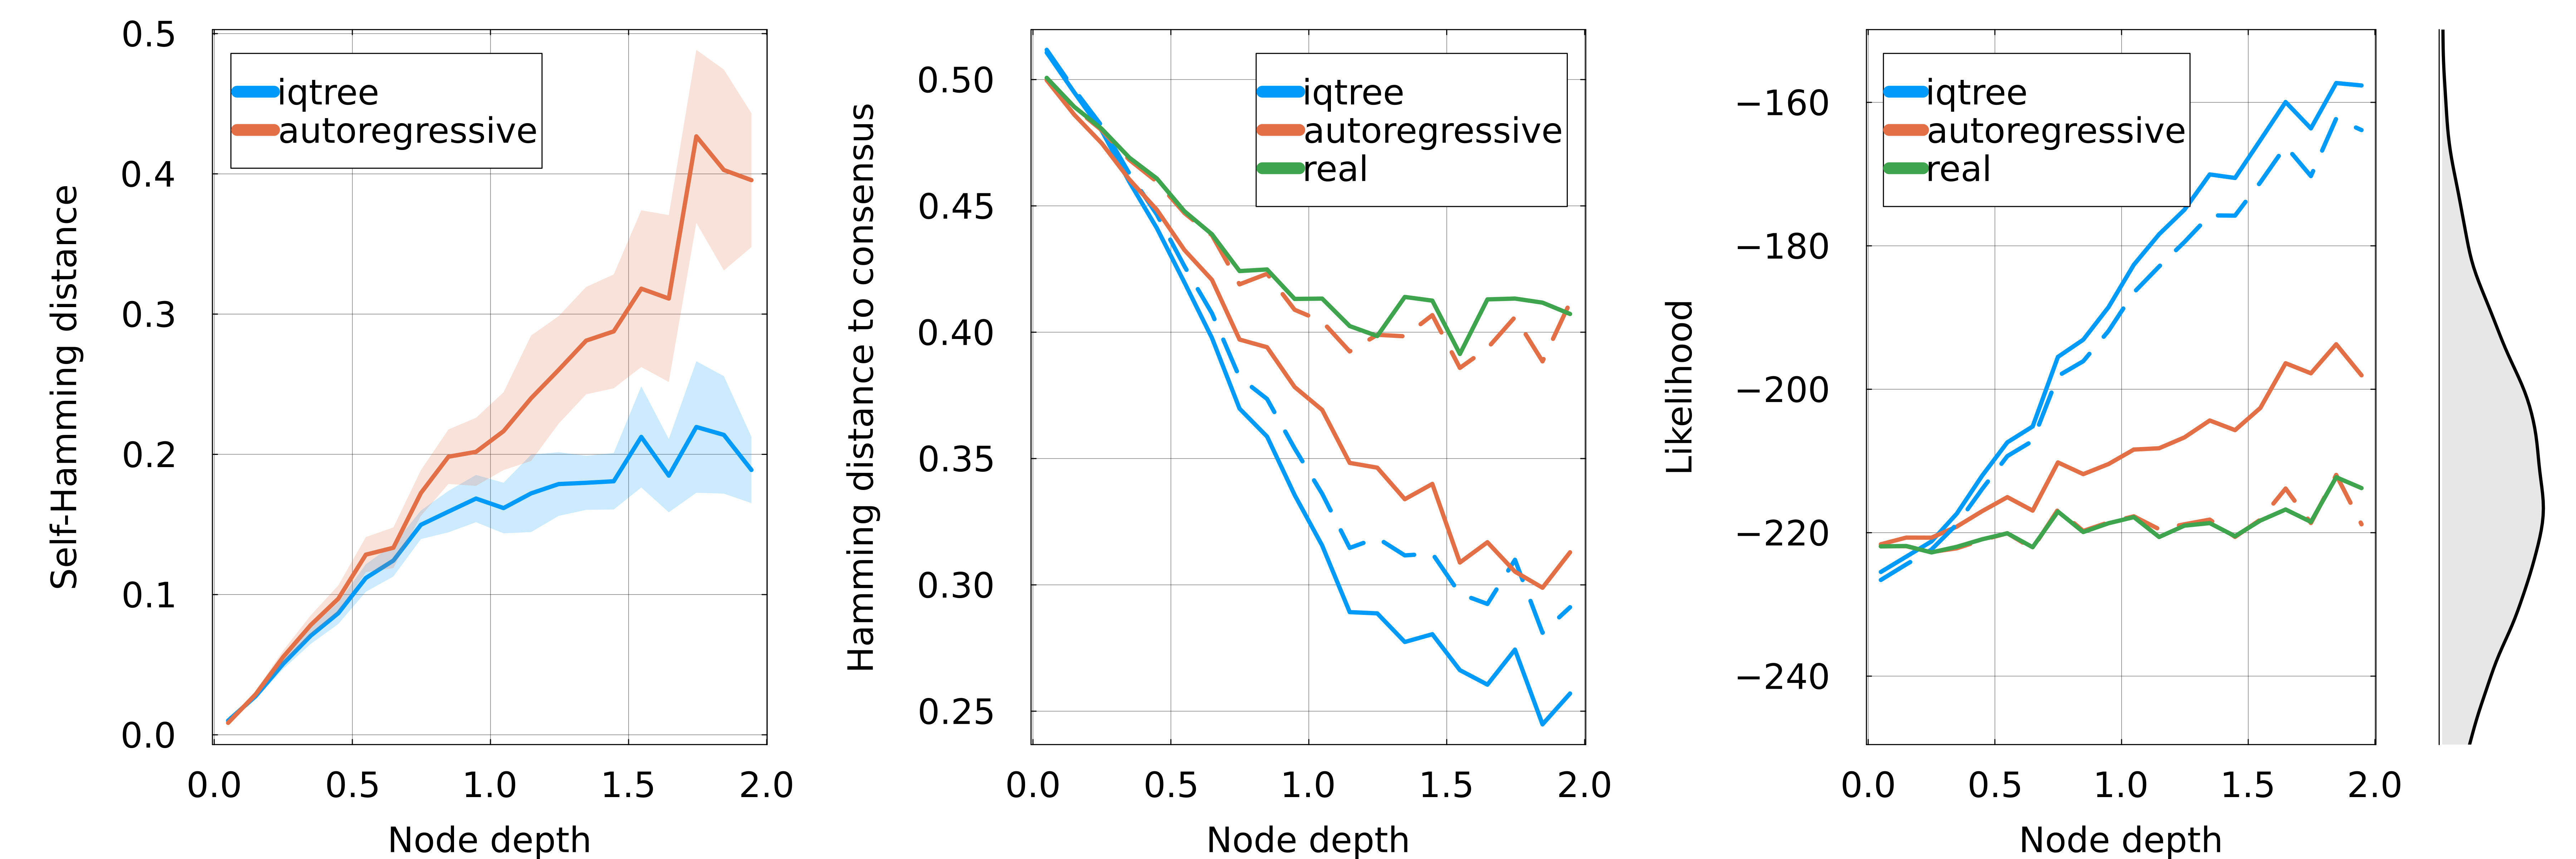
\includegraphics[width = \textwidth]{figures/diversity_likelihood_arnet_PF00072.png}
	\caption{
		\textbf{Left}: for Bayesian reconstruction, average pairwise Hamming distance among sequences reconstructed for each internal node. This quantifies the diversity of sequences obtained using Bayesian reconstruction. 
		\textbf{Center}: Hamming distance between reconstructed sequences and the consensus sequence of the alignment. Solid lines represent maximum likelihood reconstruction or the real internal sequences, and dashed lines Bayesian reconstruction. IQ-TREE appears more biased towards the consensus sequence. 
		\textbf{Right}: Log-likelihood of reconstructed and real sequences in the autoregressive model, \emph{i.e.} using the logarithm of \eqref{eq:autoregressive_def}. 
		Maximum likelihood methods (orange and blue solid lines) are biased towards more probable sequences. 
		Bayesian autoregressive reconstruction gives sequences that are at the same likelihood level than the real ancestors. The equilibrium distribution of likelihood of sequences generated by \eqref{eq:autoregressive_def} is shown on the right. 
	}
	\label{fig:diversity_likelihood_arnet}
\end{figure}

\paragraph*{Reconstructed sequences.} To further analyze the reconstructed sequences, we first look at the diversity of generated ancestors in Bayesian reconstruction. 
The left panel of \figref{fig:diversity_likelihood_arnet} shows the average Hamming distance between sequences reconstructed at the same internal node, as a function of depth. 
For deeper nodes (depth $\gtrsim 1$), the Bayesian autoregressive approach reconstructs a significantly more diverse set of sequences than IQ-TREE: Hamming distance between reconstructions saturates at $0.2$ for the latter, while it steadily increases for the former. 
Higher diversity can be interpreted as a greater uncertainty concerning the ancestral sequence. 
However, this must be put in the context of \figref{fig:hamming_real_arnet}: sequences obtained by Bayesian autoregressive reconstruction are more varied but also on average closer to the real ancestor. 

The difference in sequence diversity for the two methods is in part explained by the central panel of \figref{fig:diversity_likelihood_arnet}, which shows the Hamming distance between reconstructed ancestors and the consensus sequence of the multiple sequence alignment at the leaves. 
It appears there that for deep nodes, IQ-TREE reconstructs sequences that are relatively similar to the consensus, with an average distance between the Bayesian reconstruction and the consensus of about $0.3$. 
Contrasting with that, results of the autoregressive method shows less bias towards the consensus with an average distance of $0.4$ for deep nodes, in line with the real ancestors. 
We also note that maximum likelihood sequences for both method are always closer to the consensus than Bayesian ones, which is a known bias of maximum likelihood \cite{williams_assessingaccuracyancestral_2006}. 

The bias induced by ignoring the equilibrium distribution of the sequences is also visible in the right panel of \figref{fig:diversity_likelihood_arnet}: it shows the log-likelihood of reconstructed and real ancestral sequences according to the generative model. 
Note that the log-likelihood here comes from the log-probability of \eqref{eq:autoregressive_def} and can be interpreted as the ``quality'' of a sequence according to the generative model. 
It is unrelated to the likelihood computed in Felsenstein's pruning algorithm. 
Reconstructions with IQ-TREE increase in likelihood when going deeper in the tree, eventually resulting in sequences that are very uncharacteristic of the equilibrium generative distribution as can be seen from the histogram on the right. 
This effect also happens with the maximum likelihood reconstruction of the autoregressive model, although to a lesser extent. 
The Bayesian autoregressive reconstruction does not suffer from this bias and reconstructs sequences with a log-likelihood that is similar to that of the real ancestors. \\

\paragraph*{Potts evolver.} We then assess the performance of our reconstruction method in the case where the evolver is a Potts model. 
Potts models are a simple type of generative model and have been used extensively to model protein sequences. 
They can be use to predict contact in three dimensional structures, effects of mutations, protein-protein interaction partners \cite{cocco_inversestatisticalphysics_2018}. 
They can be sampled to generate novel sequences which are statistically similar to natural ones and often functional \cite{russ_evolutionbasedmodeldesigning_2020,mcgee_generativecapacityprobabilistic_2021}.
Additionally, it has recently been shown that they can be used to describe the evolution of protein sequences both qualitatively and quantitatively \cite{bisardi_modelingsequencespaceexploration_2021}.

Potts and autoregressive models both accurately reproduce the statistical properties of protein families. 
In this sense, it can be considered that they correspond to similar long term generative distributions in the sense of \eqref{eq:autoregressive_long_term}. 
However, the dynamics of a Potts model are fundamentally different from the ones of usual evolutionary models, including our autoregressive one. 
First, they are described by a \emph{discrete} time Markov chain, instead of the continuous time used in models based on substitution rate matrices such as in \eqref{eq:Q_decomposition} \cite{alvarez_vivofunctionalphenotypes_2024}. 
The discrete time in these dynamics corresponds to attempts at mutation, which can be either accepted or rejected depending on the effect of the mutation according to the model. 
Secondly, these dynamics naturally give rise to different evolutionary timescales for various sequence positions, as well as interesting qualitative behavior such as the entrenchment of mutations. 


\begin{figure}
	\centering
	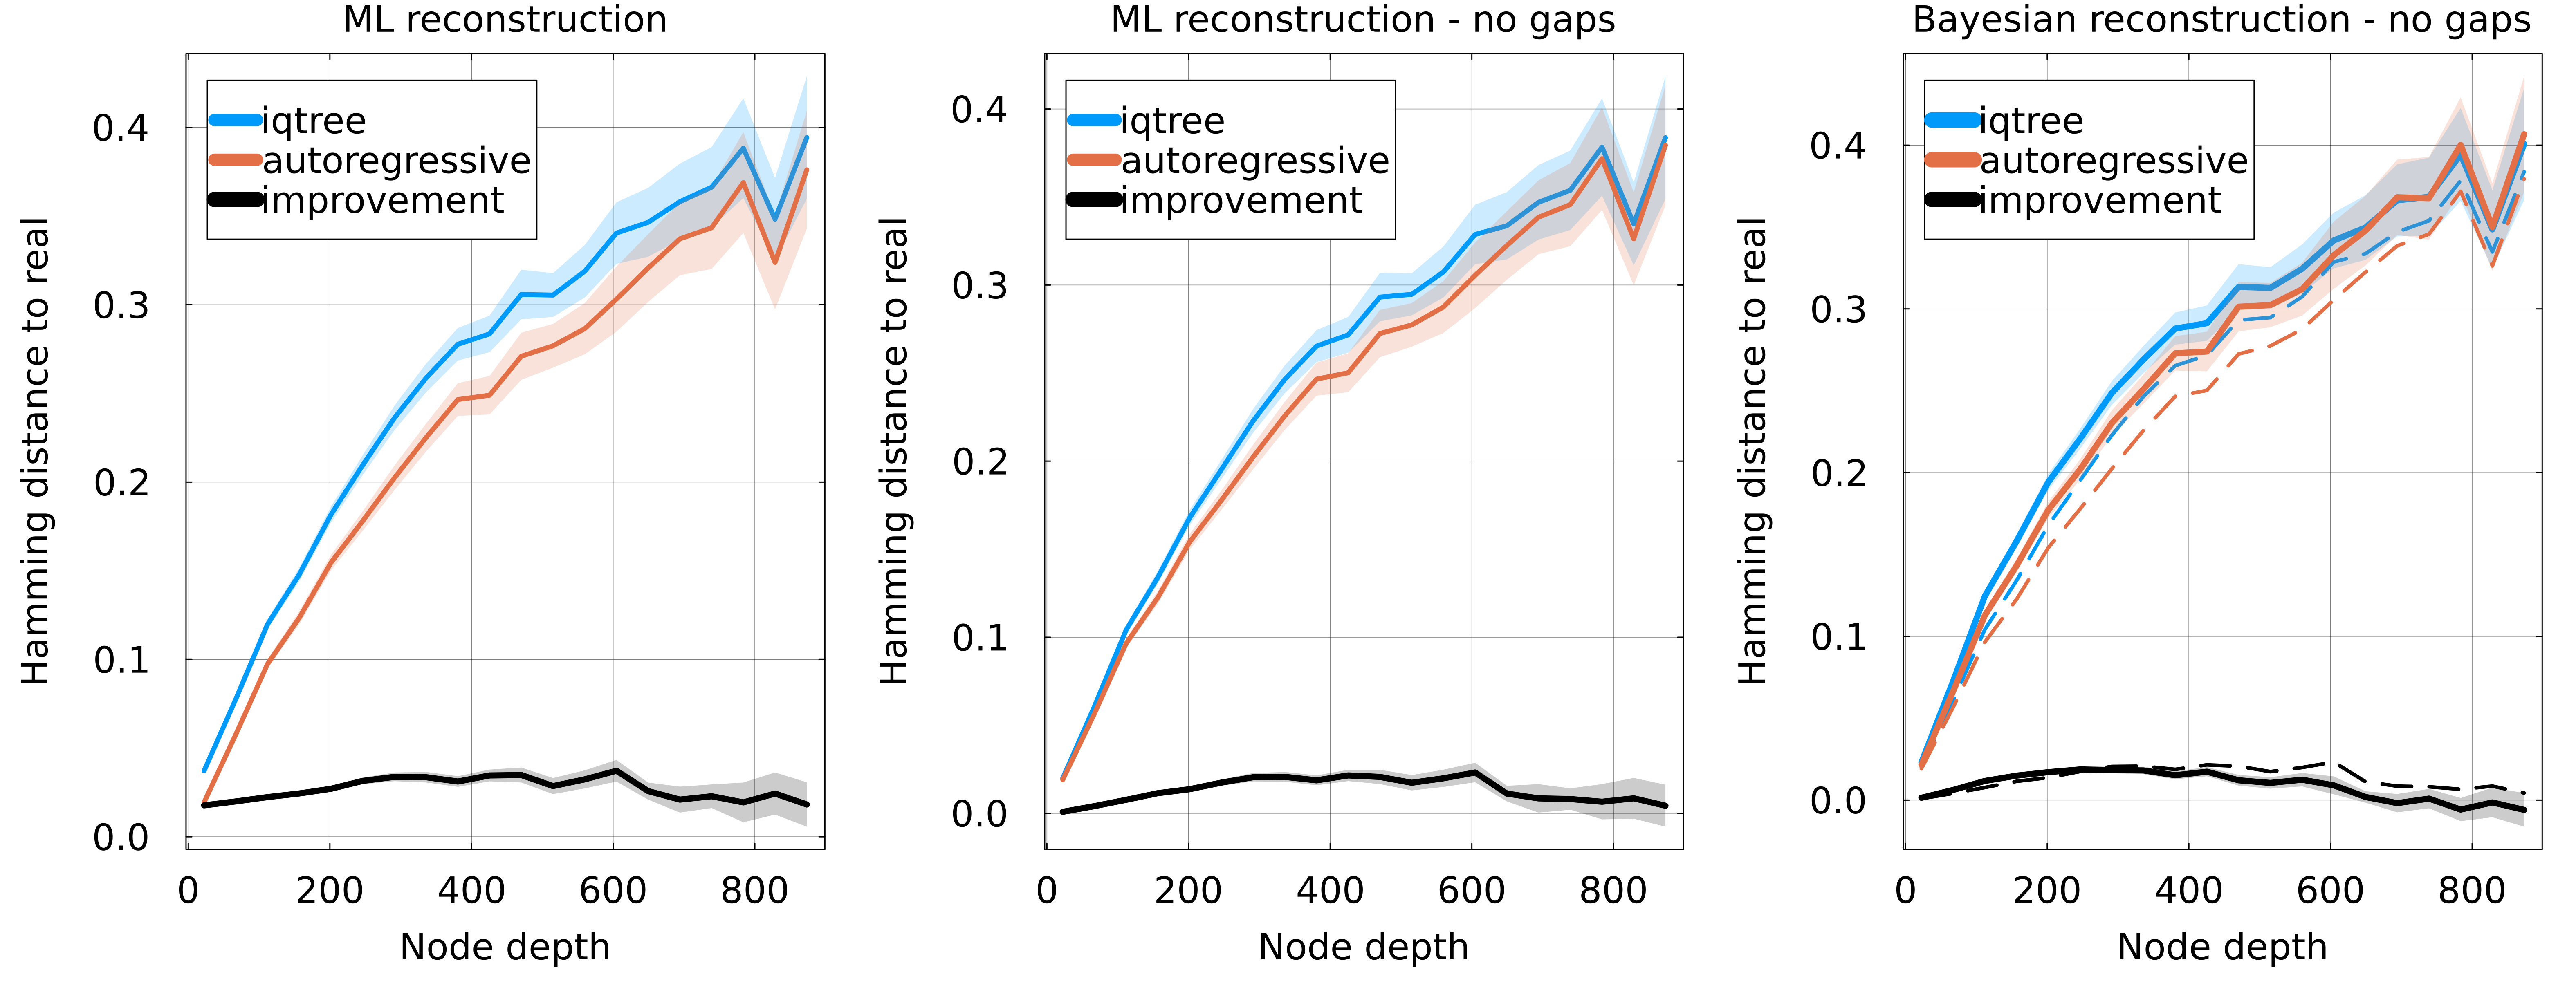
\includegraphics[width = \textwidth]{figures/hamming_to_real_potts_PF00072.png}
	\caption{
		Analogous to Figure~\ref{fig:hamming_real_arnet}, but using a Potts model as the evolver. 
		Hamming distance between reconstructed and real sequences as a function of node depth, using IQ-TREE and our autoregressive approach. 
		The difference between the two methods is shown as a black curve. 
		The evolver and reconstruction autoregressive models are learned on the PF00072 family. 
		\textbf{Left}: Hamming distance between the full aligned sequences, gaps included, using maximum likelihood reconstruction.  	
		\textbf{Center}: Hamming distance ignoring gapped positions, using maximum likelihood reconstruction. 
		\textbf{Right}: comparison of Bayesian (solid lines) and maximum likelihood (dashed lines) reconstructions, ignoring gaps. 
	}
	\label{fig:hamming_real_potts}
\end{figure}

To see how this change in dynamics affects our results, we \emph{(i)} sample a large and varied ensemble of sequences from the Potts model and use it to train an autoregressive model, in a way to guarantee consistent long term distributions between the Potts and autoregressive, and \emph{(ii)} evolve the Potts model along random phylogenies, generating alignments for the leaves and the internal nodes in the same way as above. 
We then attempt reconstruction of internal nodes using the inferred autoregressive model and IQ-TREE.
\figref{fig:hamming_real_potts} shows the results of reconstruction, with panels directly comparable to \figref{fig:hamming_real_arnet}. 
We again see a consistent improvement when using the autoregressive model over IQ-TREE, although of a much smaller amplitude, with an absolute improvement gain in Hamming distance of about 2\% for deep internal nodes.


\subsection{Results on experimental evolution data.}

We take advantage of recent developments in directed evolution experiments to test our method in a controlled setting. 
We use the data published in \cite{stiffler_proteinstructureexperimental_2020}: in this work, authors evolved the antibiotic resistant proteins $\beta$-lactamase PSE-1 and acetyltransferase AAC6 by submitting them to  cycles of mutagenesis and functional selection. 
Starting from a wild-type protein, they obtained thousands of diverse functional sequences after the directed evolution. 
An interesting result of this work is that it is possible to recover structural information about the wild-type from the set of evolved sequences. 

Here, we use this data as a test setting for ASR: the sequences obtained after directed evolution all derive from a common ancestor, the wild-type, for which we know the amino acid sequence. 
We can thus reconstruct the wild-type sequence using different ASR methods and compare it to the ground truth. 
The phylogeny is not known, but given the large populatin size during the experiment and the relatively low number of selection rounds, it is reasonable to approximate it using a star-tree, \emph{i.e.} a tree with a single coalescent event taking place at the root (see Methods). 
Since the reconstruction task is most interesting when using relatively varied sequences, we decide to use data for the PSE-1 wild-type where $20$ cycles of mutagenesis \& selection have been performed, resulting in a mean Hamming distance of $12\%$ to the wild-type. 

Our ASR procedure is as follows. 
We randomly pick $M$ amino acid sequences among the proteins evolved from PSE-1 and with $20$ cycles of mutagenesis \& selection, with $3 \leq M \leq 640$. 
The total number of sequences at round $20$ of directed evolution is much larger, making it computationally hard to use all of them. 
We then construct a star-like phylongeny and place the $M$ selected sequences at the leaves, and perform ASR using either IQ-TREE or our autoregressive method which we have trained on an alignment of PSE-1 homologs.
We obtain the reconstructed amino acid sequence of the root, which we can then compare to the actual wild-type. 
As a comparison, and because our approximation of the phylogeny is very simple, we also attempt to reconstruct the root by taking the consensus sequence of the $M$ leaves. 
We repeat this procedure $100$ times for each value of $M$ for a statistical assessment of the different methods. 

The results are shown in \figref{fig:stiffler}. 
The left panel shows the average non-normalized Hamming distance to the wild-type as a function of the number of leaves used $M$. 
For a low $M$, all methods understandably make a large number of errors, with a mean Hamming distance larger than $10$ for $M=3$. 
For a higher $M$, IQ-TREE and the autoregressive method stabilize to a fixed number of errors: we find a Hamming distance of $\sim 4.3$ for IQ-TREE and $\sim 2.9$ for the autoregressive. 
The consensus curiously reaches a minimum at intermediate $M$, a fact commented in the \SI, and saturates at a Hamming distance of $6$ when considering all sequences of the round $20$. 
The reconstruction errors are overwhelmingly located at six sequence positions. 
In the central panel, the fraction of mistakes made at these six positions over the $100$ repetitions of $M=640$ leaves is shown for each method. 
We observe that there are two positions (129 and 152) where IQ-TREE systematically fails at recovering the wild-type state while the autoregressive model's reconstruction is correct. 
Inversely, IQ-TREE recovers the wild-type state more often at position 68. 
The right panel shows the logo of the set of reconstructed sequences at these 6 positions and for each method. 

Overall, we see that the reconstruction of the autoregressive model is more accurate. 
This gain in accuracy comes from the representation of the functional constraints acting on the PSE-1 protein by the generative model, which are inferred separately using an alignment of homologs.  
The improvement in reconstruction errors is modest, going from an average Hamming distance of $4.3$ to $2.9$. 
However, the gain is intrisically limited by the data itself: the evolved sequences have an average Hamming distance of about $12\%$ to the ancestor, which is experimentally challenging but remains small compared to the divergence found in the homologs of PSE-1. 
For instance, the root-to-tip distance estimated by IQ-TREE and the autoregressive model are respectively $0.13$ and $0.15$, corresponding to the regime of shallow trees when comparing with \figref{fig:hamming_real_arnet}.


\begin{figure}
	\centering
	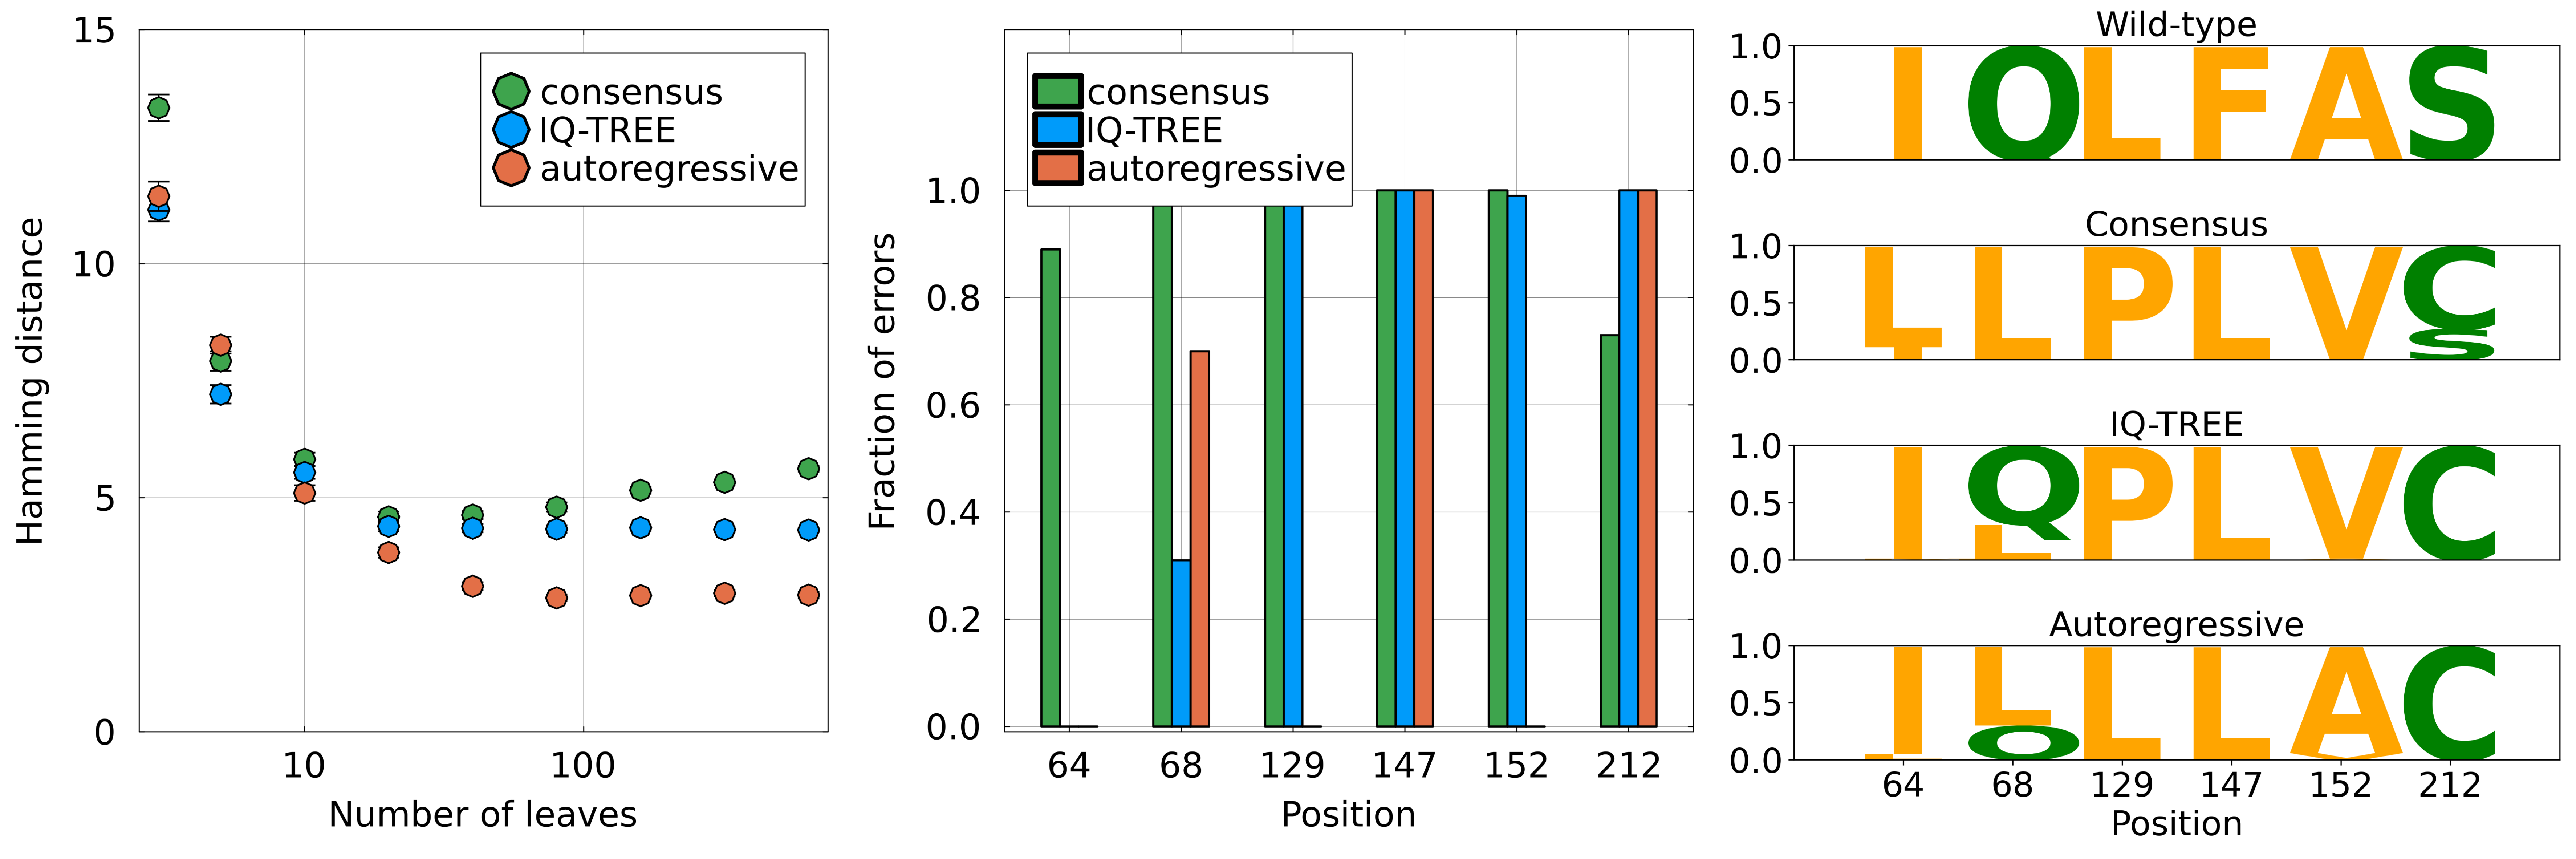
\includegraphics[width = \textwidth]{figures/stiffler_reconstruction.png}
	\caption{
		Reconstruction of the wild-type PSE1 sequence used in \cite{stiffler_proteinstructureexperimental_2020} using sequences from round $20$ of the directed evolution. 
		\textbf{Left.} Non normalized Hamming distance to the wild-type PSE1 sequence as a function of the number of sequences $M$ used for reconstruction. The fact that the consensus method has a local minimum is discussed in the \SI. For comparison, the average distance between a leaf sequence and the wild-type is $25$.
		The error bars are computed using the standard deviation obtained from the $100$ choices of sequences. 
		\textbf{Middle.} For the six sequence positions where most of the reconstruction errors are located, fraction of errors of each method out of $100$ independent reconstructions using different sets of $M = 640$ leaves. 
		\textbf{Right.} Sequence logo of the reconstructed sequence for the three methods, obtained using $100$ independent reconstructions with different sets of $M = 640$ leaves. The logo is only shown for the six positions where most errors are located. 
		For example, all three methods fail $100$ times at position $147$, reconstructing a leucine $L$ instead of a phenylalanine $F$.
	}
	\label{fig:stiffler}
\end{figure}

In order 

\section{Discussion}

\section{Methods} % (fold)
\label{sub:methods}

\subsection{ArDCA}

The ArDCA model assigns a probability to any sequence of amino acids of length $L$ given by 

\begin{equation}
	\label{eq:autoregressive_def_methods}
	P^{AR}(\mathbf{a}) = \prod_{i \in \sigma(L)} p_i(a_i \vert a_{<i}),
\end{equation}

where $\sigma(L)$ is a permutation of the $L$ first integers and $a_{<i}$ stands for $a_1, \ldots, a_{i-1}$. 
This means that the order in which the conditional probabilities $p_i$ are applied is not necessarily the sequence order. 
The permutation $\sigma$ is fixed at model inference. 

Conditional probabilities $p_i$ are defined as

\begin{equation}
	p_i(b \vert a_{<i}) = \frac{1}{Z_i}\exp\left( \sum_{j < i} J_{ij}(b, a_j) + h_i(b) \right),
\end{equation}

with the $i$ $q$-dimensional vectors $J_{i\cdot}$ and $h_i$ are learned parameters. 
The model is normally trained using a multiple sequence alignment of homologous proteins, \emph{i.e.} a protein family, by finding the parameters $J$ and $h$ that maximize the likelihood of the sequences. 
It was shown in \cite{trinquier_efficientgenerativemodeling_2021} that this specific parametrization captures essential features of the variability of members of a protein family.

By definition, homologous proteins share a joint evolutionary history and cannot be considered as statistically independent. 
To avoid biases, a reweighting is applied to sequences based on their vicinity to other sequences. 
This scheme has been showed to substantially increase the performance of such models \cite{cocco_inversestatisticalphysics_2018}. 

\subsection{Branch length inference}

\begin{itemize}
	\item how it works generally
	\item why I can't use AR directly
	\item how we do it with the profile model
	\item refer to the SI figure for results
\end{itemize}

\subsection{Simulations}

A simulation is performed as follows. 
First, a random tree of $n=100$ leaves is generated from Yule's coalescent. 
We then normalize its height to a fixed value $H$ that depends on the evolver model used: for the autoregressive model we use $H=2.0$, while for the Potts model combined with Metropolis steps, we use $H=8$ sweeps, \emph{i.e.} $H=8 L$ Metropolis steps where $L$ is the length of the sequences. 

A root sequence is sampled from the evolver model's equilibrium distribution, and evolution is simulated along each branch independently starting from the root. 
In the case of the autoregressive evolve, the dynamics is the one of \eqref{eq:autoregressive_propagator_full}. 
In the case of the Potts model, we use a Markov chain with the Metropolis update rule. 
In this way, we obtain for each repetition a tree and the alignments for internal and leaf nodes. 
Results presented in this work are obtained by averaging over $M=100$ such simulations for each protein family. 

\subsection{Experimental evolution data}

We use the data coming from the experimental evolution of the PSE-1 protein, published in \cite{stiffler_proteinstructureexperimental_2020}. 

\begin{itemize}
	\item A word on the wild-type and what it does
	\item A brief summary of the experiment. What diversity is obtained after 20 rounds? What is the population size?
	\item what the corresponding pfam is, where we got the sequences (ref.)
	\item the alignment methodology
\end{itemize}

It has been noticed in \cite{bisardi_modelingsequencespaceexploration_2021} that taking into account the transition possibilities between amino acids allowed by the genetic code is important when describing short term evolutionary dynamics with generative models. 
In our framework, a natural way to include these is by using the symetric matrix $\mathbf{H}$ in the decomposition of \eqref{eq:Q_decomposition}. 
Terms of the $\mathbf{H}$ matrix do not affect the equilibrium distribution of the model, which thus remains generative, but influences the short term dynamics. 
Here, we simply counted the number of possibilities to transition from any amino acid to any other based on the genetic code, and we constructed the corresponding $\mathbf{H}$ matrix. 
The diagonal matrix remains given by the equilibrium probabilities of amino acids in the context of the sequence, as given by \eqref{eq:autoregressive_site_propagator}.
We found that this substantially improves the results of the autoregressive reconstruction for the experimental evolution data.

\subsection{iqtree}

% iqtree2 -asr -s $aln -te $tree -pre $(tot_prefix) --keep-ident -redo

We run IQ-TREE using the \texttt{-asr}

\begin{itemize}
	\item how I run iqtree + results of model finder
\end{itemize}



\newpage
\bibliographystyle{unsrtnat}
\bibliography{references}

\newpage
\newpage
\appendix
\setcounter{figure}{0}
\renewcommand{\figurename}{Figure S}
\setcounter{table}{0}
\renewcommand{\tablename}{Table S}
\onecolumngrid

Supplementary information

\end{document}

